%definira klasu dokumenta 
\documentclass[12pt]{report} 

%prostor izmedu naredbi \documentclass i \begin{document} se zove uvod. U njemu se nalaze naredbe koje se odnose na cijeli dokument

%osnovni LaTex ne može riješiti sve probleme, pa se koriste različiti paketi koji olakšavaju izradu željenog dokumenta
\usepackage[croatian]{babel} 
\usepackage{amssymb}
\usepackage{amsmath}
\usepackage{txfonts}
\usepackage{mathdots}
\usepackage{titlesec}
\usepackage{array}
\usepackage{lastpage}
\usepackage{etoolbox}
\usepackage{tabularray}
\usepackage{color, colortbl}
\usepackage{adjustbox}
\usepackage{geometry}
\usepackage[classicReIm]{kpfonts}
\usepackage{hyperref}
\usepackage{fancyhdr}

\usepackage{float}
\usepackage{setspace}
\restylefloat{table}


\patchcmd{\chapter}{\thispagestyle{plain}}{\thispagestyle{fancy}}{}{} %redefiniranje stila stranice u paketu fancyhdr

%oblik naslova poglavlja
\titleformat{\chapter}{\normalfont\huge\bfseries}{\thechapter.}{20pt}{\Huge}
\titlespacing{\chapter}{0pt}{0pt}{40pt}


\linespread{1.3} %razmak između redaka

\geometry{a4paper, left=1in, top=1in,}  %oblik stranice

\hypersetup{ colorlinks, citecolor=black, filecolor=black, linkcolor=black,	urlcolor=black }   %izgled poveznice


%prored smanjen između redaka u nabrajanjima i popisima
\newenvironment{packed_enum}{
	\begin{enumerate}
		\setlength{\itemsep}{0pt}
		\setlength{\parskip}{0pt}
		\setlength{\parsep}{0pt}
	}{\end{enumerate}}

\newenvironment{packed_item}{
	\begin{itemize}
		\setlength{\itemsep}{0pt}
		\setlength{\parskip}{0pt}
		\setlength{\parsep}{0pt}
	}{\end{itemize}}




%boja za privatni i udaljeni kljuc u tablicama
\definecolor{LightBlue}{rgb}{0.9,0.9,1}
\definecolor{LightGreen}{rgb}{0.9,1,0.9}

%Promjena teksta za dugačke tablice
\DefTblrTemplate{contfoot-text}{normal}{Nastavljeno na idućoj stranici}
\SetTblrTemplate{contfoot-text}{normal}
\DefTblrTemplate{conthead-text}{normal}{(Nastavljeno)}
\SetTblrTemplate{conthead-text}{normal}
\DefTblrTemplate{middlehead,lasthead}{normal}{Nastavljeno od prethodne stranice}
\SetTblrTemplate{middlehead,lasthead}{normal}

%podesavanje zaglavlja i podnožja

\pagestyle{fancy}
\lhead{Programsko inženjerstvo}
\rhead{Nestali ljubimci}
\lfoot{MP7}
\cfoot{stranica \thepage/\pageref{LastPage}}
\rfoot{\today}
\renewcommand{\headrulewidth}{0.2pt}
\renewcommand{\footrulewidth}{0.2pt}


\begin{document} 
	
	
	
	\begin{titlepage}
		\begin{center}
			\vspace*{\stretch{1.0}} %u kombinaciji s ostalim \vspace naredbama definira razmak između redaka teksta
			\LARGE Programsko inženjerstvo\\
			\large Ak. god. 2023./2024.\\
			
			\vspace*{\stretch{3.0}}
			
			\huge Nestali ljubimci\\
			\Large Dokumentacija, Rev. \textit{1}\\
			
			\vspace*{\stretch{12.0}}
			\normalsize
			Grupa: \textit{MP7}\\
			Voditeljica: \textit{Mia Krstičević}\\
			
			
			\vspace*{\stretch{1.0}}
			Datum predaje: \textit{$<$dan$>$. $<$mjesec$>$. $<$godina$>$.}\\
	
			\vspace*{\stretch{4.0}}
			
			Nastavnik: \textit{Alan Jović}\\
		
		\end{center}

	
	\end{titlepage}

	
	\tableofcontents


	\chapter{Dnevnik promjena dokumentacije}
		
		\textbf{\textit{Kontinuirano osvježavanje}}\\
				
		
		\begin{longtblr}[
				label=none
			]{
				width = \textwidth, 
				colspec={|X[2]|X[13]|X[3]|X[3]|}, 
				rowhead = 1
			}
			\hline
			\textbf{Rev.}	& \textbf{Opis promjene/dodatka} & \textbf{Autori} & \textbf{Datum}\\[3pt] \hline
			0.1 & Napravljena shema baze podataka.	& Mia \newline Krstičević & 27.10.2023. 		\\[3pt] \hline 
			0.2	& Napravljen predložak projektne dokumentacije i dodan opis projektnog zadatka. Dopisane upute za povijest dokumentacije.\newline & Lucija Renić & 28.10.2023. 	\\[3pt] \hline 
			0.3 & U specifikaciju programske potpore dodani funkcionalni zahtjevi.  Dodani Ostali zahtjevi i Obrasci uporabe  & Lucija Renić & 30.10.2023. \\[3pt] \hline 
			0.4 & Nova verzija baze podataka & Mia \newline Krstičević & 05.11.2023. \\[3pt] \hline 
			0.5 & Uređen opis projektnog zadatka \newline Dodan opis baze & Mia \newline Krstičević  & 07.11.2023. \\[3pt] \hline 
			0.6.1 & Dodan dijagram baze podataka & Mia \newline Krstičević & 09.11.2023. \\[3pt] \hline 
			0.6.2 & Dodan UML dijagram obrasca uporabe & Toni Vanjak, Lucija Renić & 09.11.2023. \\[3pt] \hline 
			0.7 & Ispravljen UML dijagram obrasca uporabe & Toni Vanjak, Lucija Renić & 11.11.2023. \\[3pt] \hline 
			0.8 & Dodani sekvencijski dijagrami & Toni Vanjak, Lucija Renić & 11.11.2023. \\[3pt] \hline 
			0.9 & Dodani opisi sekvencijskih dijagrama & Lucija Renić & 15.11.2023. \\[3pt] \hline 
			0.10 & Dodan opis arhitekture & Toni Vanjak & 16.11.2023. \\[3pt] \hline 
			0.11 & Ispravljen sekvencijski dijagram UC7 & Toni Vanjak & 17.11.2023. \\[3pt] \hline
			0.12 & Dodan UC15 i popravljen dijagram obrazaca uporabe & Toni Vanjak, Mia \newline Krstičevič, Lucija Renić & 17.11.2023. \\[3pt] \hline
			0.13 & Uređen opis projektnog zadatka & Mia \newline Krstičević, Lucija Renić & 17.11.2023. \\[3pt] \hline
			0.14 & Ispravljen sekvencijski dijagram UC3 & Toni Vanjak & 17.11.2023. \\[3pt] \hline
			0.15 & Dodan dijagram razreda & Toni Vanjak & 17.11.2023. \\[3pt] \hline
			%\textbf{1.0} & Verzija samo s bitnim dijelovima za 1. ciklus & * & 11.09.2013. \\[3pt] \hline 
			%1.1 & Uređivanje teksta -- funkcionalni i nefunkcionalni zahtjevi & * \newline * & 14.09.2013. \\[3pt] \hline 
			%1.2 & Manje izmjene:Timer - Brojilo vremena & * & 15.09.2013. \\[3pt] \hline 
			%1.3 & Popravljeni dijagrami obrazaca uporabe & * & 15.09.2013. \\[3pt] \hline 
			%1.5 & Generalna revizija strukture dokumenta & * & 19.09.2013. \\[3pt] \hline 
			%1.5.1 & Manja revizija (dijagram razmještaja) & * & 20.09.2013. \\[3pt] \hline 
			%\textbf{2.0} & Konačni tekst predloška dokumentacije  & * & 28.09.2013. \\[3pt] \hline 
			%&  &  & \\[3pt] \hline	
		\end{longtblr}
	
	
		%\textit{Moraju postojati glavne revizije dokumenata 1.0 i 2.0 na kraju prvog i drugog ciklusa. Između tih revizija mogu postojati manje revizije već prema tome kako se dokument bude nadopunjavao. Očekuje se da nakon svake značajnije promjene (dodatka, izmjene, uklanjanja dijelova teksta i popratnih grafičkih sadržaja) dokumenta se to zabilježi kao revizija. Npr., revizije unutar prvog ciklusa će imati oznake 0.1, 0.2, …, 0.9, 0.10, 0.11.. sve do konačne revizije prvog ciklusa 1.0. U drugom ciklusu se nastavlja s revizijama 1.1, 1.2, itd.}
	\chapter{Opis projektnog zadatka}
		
		%\textbf{\textit{dio 1. revizije}}\\
		
		%\textit{Na osnovi projektnog zadatka detaljno opisati korisničke zahtjeve. Što jasnije opisati cilj projektnog zadatka, razraditi problematiku zadatka, dodati nove aspekte problema i potencijalnih rješenja. Očekuje se minimalno 3, a poželjno 4-5 stranica opisa.	Teme koje treba dodatno razraditi u ovom poglavlju su:}\\
		%\underline{CILJ}\\
		Cilj ovog projektnog zadatka je razviti web aplikaciju „Nestali ljubimci“ koja će korisniku olakšati potragu za odlutalim kućnim ljubimcem. Budući da je informacije o potrazi nepraktično oglašavati putem uobičajenih internetskih platformi za komunikaciju (npr. društvene mreže, stranice za oglašavanje, forumi i slično), ova web aplikacija će vlasnicima životinja, skloništima za životinje i dobrim ljudima koji pomažu u pronalasku životinje omogućiti brz i efikasan način izmjene informacija o nestanku, opažanju i pronalasku odbjeglog kućnog ljubimca. U ime što bržeg pronalaska ljubimca, web aplikacija će biti razvijena za mobilne uređaje  kako bi u procesu potrage podržala veću brzinu reagiranja, koja je često ključna za uspješan završetak potrage za kućnim ljubimcem.\\
		
		Prilikom ulaska u web aplikaciju prikazuju se aktivni oglasi i oglasi o životinjama koje su pronašla skloništa.\\
		
		\textbf{KORISNICI}\\
		Aplikacija podržava rad tri tipa korisnika (neregistrirani korisnik, registrirani korisnik i sklonište za životinje).\\
		\underline{Neregistrirani korisnik} pri ulasku u web aplikaciju ima mogućnost pregledavati i pretraživati aktivne oglase o nestalim kućnim ljubimcima i oglase skloništa za životinje. Pretraživanje je ostvareno po nazivu skloništa i po kategorijama podataka o ljubimcu koje su dostupne pri oglašavanju (vrsta, ime na koje se odaziva, datum i sat nestanka, lokacija nestanka, boja, starost, tekstni opis). Za detaljniji pregled informacija o kućnom ljubimcu kao i pregled komunikacije o potrazi za njime potrebno je odabrati oglas. Ako neregistrirani korisnik može i želi doprinijeti potrazi davanjem nekih informacija, potrebna je registracija.
		Podaci potrebni za registraciju su:
		\begin{packed_item}
			\item Ime
			\item Ime
			\item Korisničko ime
			\item Lozinka
			\item Adresa e-pošte
			\item Broj telefona
	    \end{packed_item}
	    \underline{Registrirani korisnik}, koji osim svih mogućnosti koje ima i neregistrirani korisnik, dodatno ima sljedeće mogućnosti:
		\begin{packed_item}
			\item Postavljanje oglasa o nestalom kućnom ljubimcu 
			\item Sudjelovanje u komunikaciji oko potrage za ljubimcem
			\item Uklanjanje oglasa o nestalom kućnom ljubimcu
			\item Izmjena oglasa o nestalom kućnom ljubimcu
		\end{packed_item}
		Treći tip korisnika su \underline{skloništa za životinje}, koji osiim svih mogućnosti koje ima registrirani korisnik, ima dodatnu mogućnost oglašavanja životinja koje su pronađene i nalaze se u njihovom prostoru. Skloništa za životinje pri registraciji moraju unijeti i naziv skloništa.\\
		
		\textbf{OGLASI}\\
		Za \underline{postavljanje oglasa} potrebno je unijeti sljedeće informacije o ljubimcu:
		\begin{packed_item}
			\item Vrsta
			\item Ime na koje se odaziva
			\item Datum i sat nestanka
			\item Lokacija nestanka
			\item Boja
			\item Starost
			\item Tekstni opis
			\item Slike (najviše 3 slike)
		\end{packed_item}
		Osim podataka o kućnom ljubimcu, oglas sadrži i kontak podatke korisnika koji se povlače iz korisničkih podataka danih pri registraciji (adresa e-pošte, broj telefona).\\
		Oglas mora imati jednu od \underline{kategorija}:
		\begin{packed_item}
			\item Za ljubimcem se traga (aktivan oglas)
			\item Ljubimac je sretno pronađen
			\item Ljubimac nije pronađen, ali se za njim više ne traga aktivno
			\item Ljubimac je pronađen uz nesretne okolnosti
			\item U skloništu (koju može postaviti samo sklonište za životinje)
		\end{packed_item}
		Na oglasu je moguća \underline{izmjena} svih kategorija podataka o ljubimcima, kao i kategorija oglasa. Sve kategorije, osim da se za ljubimcem aktivno traga, oglas čine neaktivnim. Popis neaktivnih oglasa mogu pregledavati samo registrirani korisnici.\\
		\underline{Komunikacija} oko potrage za kućnim ljubimcem odvijat će se porukama koje mogu sadržavati:
		\begin{packed_item}
			\item Tekst
			\item Sliku
			\item Geolokaciju
		\end{packed_item}
		uz kontakt podatke o osobi koja komunicira.\\
		
		\textbf{Ostalo}\\
		Aplikacija je izvedena kao mobilna aplikacija.\\
		Sustav podržava rad više korisnika u stvarnom vremenu.\\
		Aplikacija je namijenjena vlasnicima životinja i svim dobrim dušama koje su volje pomoći oko potrage za nestalim kućnim ljubimcima.
		%\begin{packed_item}
			%\item \textit{potencijalna korist ovog projekta}
			%\item \textit{postojeća slična rješenja (istražiti i ukratko opisati razlike u odnosu na zadani zadatak). Dodajte slike koja predočavaju slična rješenja.}
			%\item \textit{skup korisnika koji bi mogao biti zainteresiran za ostvareno rješenje.}
			%\item \textit{mogućnost prilagodbe rješenja }
			%\item \textit{opseg projektnog zadatka}
			%\item \textit{moguće nadogradnje projektnog zadatka}
		%\end{packed_item}
		
		%\textit{Za pomoć pogledati reference navedene u poglavlju „Popis literature“, a po potrebi konzultirati sadržaj na internetu koji nudi dobre smjernice u tom pogledu.}
		\eject
		
		\section{Primjeri u \LaTeX u}
		
		\textit{Ovo potpoglavlje izbrisati.}\\

		U nastavku se nalaze različiti primjeri kako koristiti osnovne funkcionalnosti \LaTeX a koje su potrebne za izradu dokumentacije. Za dodatnu pomoć obratiti se asistentu na projektu ili potražiti upute na sljedećim web sjedištima:
		\begin{itemize}
			\item Upute za izradu diplomskog rada u \LaTeX u - \url{https://www.fer.unizg.hr/_download/repository/LaTeX-upute.pdf}
			\item \LaTeX\ projekt - \url{https://www.latex-project.org/help/}
			\item StackExchange za Tex - \url{https://tex.stackexchange.com/}\\
		
		\end{itemize} 	


		
		\noindent \underbar{podcrtani tekst}, \textbf{podebljani tekst}, 	\textit{nagnuti tekst}\\
		\noindent \normalsize primjer \large primjer \Large primjer \LARGE {primjer} \huge {primjer} \Huge primjer \normalsize
				
		\begin{packed_item}
			
			\item  primjer
			\item  primjer
			\item  primjer
			\item[] \begin{packed_enum}
				\item primjer
				\item[] \begin{packed_enum}
					\item[1.a] primjer
					\item[b] primjer
				\end{packed_enum}
				\item primjer
			\end{packed_enum}
			
		\end{packed_item}
		
		\noindent primjer url-a: \url{https://www.fer.unizg.hr/predmet/proinz/projekt}
		
		\noindent posebni znakovi: \# \$ \% \& \{ \} \_ 
		$|$ $<$ $>$ 
		\^{} 
		\~{} 
		$\backslash$ 
		
		
		\begin{longtblr}[
			label=none,
			entry=none
			]{
				width = \textwidth,
				colspec={|X[8,l]|X[8, l]|X[16, l]|}, 
				rowhead = 1,
			} %definicija širine tablice, širine stupaca, poravnanje i broja redaka naslova tablice
			\hline \SetCell[c=3]{c}{\textbf{naslov unutar tablice}}	 \\ \hline[3pt]
			\SetCell{LightGreen}IDKorisnik & INT	&  	Lorem ipsum dolor sit amet, consectetur adipiscing elit, sed do eiusmod  	\\ \hline
			korisnickoIme	& VARCHAR &   	\\ \hline 
			email & VARCHAR &   \\ \hline 
			ime & VARCHAR	&  		\\ \hline 
			\SetCell{LightBlue} primjer	& VARCHAR &   	\\ \hline 
		\end{longtblr}
		

		\begin{longtblr}[
				caption = {Naslov s referencom izvan tablice},
				entry = {Short Caption},
			]{
				width = \textwidth, 
				colspec = {|X[8,l]|X[8,l]|X[16,l]|}, 
				rowhead = 1,
			}
			\hline
			\SetCell{LightGreen}IDKorisnik & INT	&  	Lorem ipsum dolor sit amet, consectetur adipiscing elit, sed do eiusmod  	\\ \hline
			korisnickoIme	& VARCHAR &   	\\ \hline 
			email & VARCHAR &   \\ \hline 
			ime & VARCHAR	&  		\\ \hline 
			\SetCell{LightBlue} primjer	& VARCHAR &   	\\ \hline 
		\end{longtblr}
	


		
		
		%unos slike
		\begin{figure}[H]
			\includegraphics[scale=0.4]{slike/aktivnost.PNG} %veličina slike u odnosu na originalnu datoteku i pozicija slike
			\centering
			\caption{Primjer slike s potpisom}
			\label{fig:promjene}
		\end{figure}
		
		\begin{figure}[H]
			\includegraphics[width=\textwidth]{slike/aktivnost.PNG} %veličina u odnosu na širinu linije
			\caption{Primjer slike s potpisom 2}
			\label{fig:promjene2} %label mora biti drugaciji za svaku sliku
		\end{figure}
		
		Referenciranje slike \ref{fig:promjene2} u tekstu.
		
		\eject
		
	
	\chapter{Specifikacija programske potpore}

\section{Funkcionalni zahtjevi}

%\textbf{\textit{dio 1. revizije}}\\

%\textit{Navesti \textbf{dionike} koji imaju %\textbf{interes u ovom sustavu} ili  \textbf{su %nositelji odgovornosti}. To su prije svega %korisnici, ali i administratori sustava, %naručitelji, razvojni tim.}\\

%\textit{Navesti \textbf{aktore} koji izravno \textbf{koriste} ili \textbf{komuniciraju sa sustavom}. Oni mogu imati inicijatorsku ulogu, tj. započinju određene procese u sustavu ili samo sudioničku ulogu, tj. obavljaju određeni posao. Za svakog aktora navesti funkcionalne zahtjeve koji se na njega odnose.}\\


\noindent \textbf{Dionici:}

\begin{packed_enum}
	
	\item Vlasnik (naručitelj)
	\item Vlasnici kućnih ljubimaca				
	\item Ljudi koji pomažu u potrazi
	\item Skloništa za životinje
	\item Razvojni tim
	
\end{packed_enum}

\noindent \textbf{Aktori i njihovi funkcionalni zahtjevi:}


\begin{packed_enum}
	\item  \underbar{Neregistrirani korisnik (inicijator) može:}
	
	\begin{packed_enum}
		
		\item registrirati se, stvoriti novi korisnički račun za koje je potrebno unijeti ime, prezime, korisničko ime, lozinku, adresu e-pošte, broj telefona
		\item pregledavati i pretraživati aktivne oglase
		\item odabrati oglas za detaljniji pregled informacija o kućnom ljubimcu i pregled komunikacije oko kućnog ljubimca
		
		
	\end{packed_enum}
	
	\item  \underbar{Vlasnik kućnog ljubimca (inicijator) može:}
	
	\begin{packed_enum}
		
		\item izbrisati korisnički račun
		\item pregledavati i mijenjati osobne podatke
		\item pregledavati aktivne i neaktivne oglase
		\item postaviti oglas o nestalom kućnom ljubimcu za koji je potrebno unijeti vrstu, ime na koje se odaziva, datum i sat nestanka, lokaciju nestanka, boju, starost, tekstni opis i slike (do 3)
		\item sudjelovati u komunikaciji o nestalom kućnom ljubimcu
		\begin{packed_enum}
			
			\item sudjelovati slanjem tekstne poruke
			\item sudjelovati slanjem slike
			\item sudjelovati slanjem geolokacije
			
		\end{packed_enum}
		\item ukloniti oglas o nestalom kućnom ljubimcu
		\item izmjenjivati oglas o nestalom kućnom ljubimcu
		
		
	\end{packed_enum}
	
	\item  \underbar{Sudionik u potrazi (inicijator) može:}
	
	\begin{packed_enum}
		
		\item izbrisati korisnički račun
		\item pregledavati i mijenjati osobne podatke
		\item pregledavati aktivne i neaktivne oglase
		\item sudjelovati u komunikaciji o nestalom kućnom ljubimcu
		\begin{packed_enum}
			
			\item sudjelovati slanjem tekstne poruke
			\item sudjelovati slanjem slike
			\item sudjelovati slanjem geolokacije
			
		\end{packed_enum}
		
	\end{packed_enum}
	\item  \underbar{Sklonište za životinje (inicijator) može:}
	
	\begin{packed_enum}
		
		\item izbrisati korisnički račun
		\item pregledavati aktivne i neaktivne oglase
		\item postaviti oglas o pronađenoj životinji
		\item sudjelovati u komunikaciji o nestalom kućnom ljubimcu
		\begin{packed_enum}
			
			\item sudjelovati slanjem tekstne poruke
			\item sudjelovati slanjem slike
			\item sudjelovati slanjem geolokacije
			
		\end{packed_enum}
		
		
	\end{packed_enum}
	
	\item  \underbar{Baza podataka (sudionik) može:}
	
	\begin{packed_enum}
		
		\item pohraniti podatke o korisnicima
		\item pohraniti podatke o kućnim ljubimcima (oglase)
		
		
		
	\end{packed_enum}
	
\end{packed_enum}

\eject 



\subsection{Obrasci uporabe}

%\textbf{\textit{dio 1. revizije}}

%\subsubsection{Opis obrazaca uporabe}
%\textit{Funkcionalne zahtjeve razraditi u obliku obrazaca uporabe. Svaki obrazac je potrebno razraditi prema donjem predlošku. Ukoliko u nekom koraku može doći do odstupanja, potrebno je to odstupanje opisati i po mogućnosti ponuditi rješenje kojim bi se tijek obrasca vratio na osnovni tijek.}\\


\noindent \underbar{\textbf{UC1 - Pregled aktivnih oglasa}}
\begin{packed_item}
	
	\item \textbf{Glavni sudionik: }Korisnik
	\item  \textbf{Cilj:} Pregledati oglase o nestalim kućnim ljubimcima
	\item  \textbf{Sudionici:} Baza podataka
	\item  \textbf{Preduvjet:} -
	\item  \textbf{Opis osnovnog tijeka:}
	
	\item[] \begin{packed_enum}
		
		\item Aktivni oglasi su prikazani prilikom učitavanja aplikacije
		\item Korisnik odabire oglas za više informacija
		\item Prikazuju se informacije i komunikacija o nestalom kućnom ljubimcu

	\end{packed_enum}
	
\end{packed_item}

\noindent \underbar{\textbf{UC2 - Registracija}}
\begin{packed_item}
	
	\item \textbf{Glavni sudionik: }Korisnik
	\item  \textbf{Cilj:} Stvoriti korisnički račun za pristup sustavu
	\item  \textbf{Sudionici:} Baza podataka
	\item  \textbf{Preduvjet:} -
	\item  \textbf{Opis osnovnog tijeka:}
	
	\item[] \begin{packed_enum}
		
		\item Korisnik odabire opciju za registraciju
		\item Korisnik unosi potrebne korisničke podatke
		\item Korisnik prima obavijest o uspješnoj registraciji

	\end{packed_enum}
	
	\item  \textbf{Opis mogućih odstupanja:}
	
	\item[] \begin{packed_item}
		
		\item[2.a] Odabir već zauzetog korisničkog imena i/ili e-maila, unos korisničkog podatka u nedozvoljenom formatu ili unos neispravnoga e-maila
		
		\item[] \begin{packed_enum}
			
			\item Sustav obavještava korisnika o pogrešnom unosu podataka i vraća ga na stranicu za registraciju
			\item Korisnik mijenja potrebne podatke te završava unos ili odustaje od registracije
			
		\end{packed_enum}

		
	\end{packed_item}
\end{packed_item}



\noindent \underbar{\textbf{UC3 - Prijava u sustav}}
\begin{packed_item}
	
	\item \textbf{Glavni sudionik: }Registrirani korisnik
	\item  \textbf{Cilj:} Dobiti pristup korisničkom sučelju
	\item  \textbf{Sudionici:} Baza podataka
	\item  \textbf{Preduvjet:}  Registracija
	\item  \textbf{Opis osnovnog tijeka:}
	
	\item[] \begin{packed_enum}
		
		\item Unos korisničkog imena i lozinke
		\item Potvrda o ispravnosti unesenih podataka
		\item Pristup korisničkim funkcijama

	\end{packed_enum}
	
	\item  \textbf{Opis mogućih odstupanja:}
	
	\item[] \begin{packed_item}
		
		\item[2.a] Neispravno korisničko ime/lozinka
		\item[] \begin{packed_enum}
			
			\item Sustav obavještava korisnika o neuspjeloj prijavi i vraća ga na stranicu za prijavu u sustav
			\item Korisnik unosi ispravne podatke i uspješno se prijavljuje u sustav
			
		\end{packed_enum}
		
	\end{packed_item}
\end{packed_item}

\noindent \underbar{\textbf{UC4 - Pregled osobnih podataka}}
\begin{packed_item}
	
	\item \textbf{Glavni sudionik: }Registrirani korisnik
	\item  \textbf{Cilj:} Pregledati osobne podatke
	\item  \textbf{Sudionici:} Baza podataka
	\item  \textbf{Preduvjet:} Korisnik je prijavljen
	\item  \textbf{Opis osnovnog tijeka:}
	
	\item[] \begin{packed_enum}
		
		\item Korisnik odabire opciju ”Osobni podatci”
		\item Aplikacija prikazuje osobne podatke korisnika

	\end{packed_enum}
	
\end{packed_item}

\noindent \underbar{\textbf{UC5 - Promjena osobnih podataka}}
\begin{packed_item}
	
	\item \textbf{Glavni sudionik: }Registrirani korisnik
	\item  \textbf{Cilj:} Promijeniti osobne podatke
	\item  \textbf{Sudionici:} Baza podataka
	\item  \textbf{Preduvjet:} Korisnik je prijavljen
	\item  \textbf{Opis osnovnog tijeka:}
	
	\item[] \begin{packed_enum}
		
		\item Korisnik odabere opciju za promjenu podataka
		\item Korisnik upisuje nove osobne podatke
		\item Korisnik sprema promjene
		\item Baza podataka sprema nove podatke
	\end{packed_enum}
	
	\item  \textbf{Opis mogućih odstupanja:}
	
	\item[] \begin{packed_item}
		
		\item[3.a] Korisnik promijeni svoje osobne podatke, ali ne odabere opciju ”Spremi promjenu”
		
		\item[] \begin{packed_enum}
			
			\item Sustav obavještava korisnika da nije spremio podatke prije izlaska iz prozora
			
		\end{packed_enum}
		
		
	\end{packed_item}
\end{packed_item}

\noindent \underbar{\textbf{UC6 - Brisanje korisničkog računa}}
\begin{packed_item}
	
	\item \textbf{Glavni sudionik: }Registrirani korisnik
	\item  \textbf{Cilj:} Izbrisati svoj korisnički račun
	\item  \textbf{Sudionici:} Baza podataka
	\item  \textbf{Preduvjet:} Korisnik je prijavljen
	\item  \textbf{Opis osnovnog tijeka:}
	
	\item[] \begin{packed_enum}
		
		\item Korisnik pregledava osobne podatke
		\item Otvara se stranica s osobnim podacima korisnika
		\item Korisnik odabire opciju „Izbriši račun“
		\item Korisnički račun briše se iz baze podataka
		\item Otvara se stranica za registraciju
	\end{packed_enum}
	
\end{packed_item}

\noindent \underbar{\textbf{UC7 - Postavljanje oglasa}}
\begin{packed_item}
	
	\item \textbf{Glavni sudionik: }Registrirani korisnik
	\item  \textbf{Cilj:} Postavljanje oglasa o nestalom kućnom ljubimcu
	\item  \textbf{Sudionici:} Baza podataka
	\item  \textbf{Preduvjet:} Korisnik je prijavljen
	\item  \textbf{Opis osnovnog tijeka:}
	
	\item[] \begin{packed_enum}
		
		\item Korisnik odabire opciju "Novi oglas"
		\item Korisnik unosi podatke o nestalom kućnom ljubimcu
		\item Korisnik odabire opciju "Postavi oglas"
	\end{packed_enum}
	
	\item  \textbf{Opis mogućih odstupanja:}
	
	\item[] \begin{packed_item}
		
		\item[3.a] Korisnik ne unosi obvezne podatke o ljubimcu
		\item[] \begin{packed_enum}
			
			\item Sustav obavještava korisnika da nisu uneseni svi potrebni podaci
			\item Korisnik unosi sve podatke
			\item Korisnik postavlja oglas
		
		
			\end{packed_enum}
			
			
		\item[3.b] Korisnik odustaje od postavljanja oglasa
		\item[] \begin{packed_enum}
			\item Sustav obavještava korisnika da oglas neće biti postavljen
			\item Prikazuje se početna stranica
		\end{packed_enum}
		
		
	\end{packed_item}
\end{packed_item}

\noindent \underbar{\textbf{UC8 - Moji oglasi}}
\begin{packed_item}
	
	\item \textbf{Glavni sudionik: }Registrirani korisnik
	\item  \textbf{Cilj:} Pregledati listu oglasa koje je postavio korisnik
	\item  \textbf{Sudionici:} Baza podataka
	\item  \textbf{Preduvjet:} Korisnik je prijavljen u sustav
	\item  \textbf{Opis osnovnog tijeka:}
	
	\item[] \begin{packed_enum}
		
		\item Korisnik odabire opciju "Moji oglasi"
		\item Aplikacija prikazuje listu oglasa koje je postavio korisnik

	\end{packed_enum}
	
	\item  \textbf{Opis mogućih odstupanja:}
	
	\item[] \begin{packed_item}
		
		\item[2.a] Korisnik nema postavljene oglase
		\item[] \begin{packed_enum}
			
			\item Sustav obavještava korisnika da još nije postavio oglas
			
		\end{packed_enum}
		
		
	\end{packed_item}
\end{packed_item}

\noindent \underbar{\textbf{UC9 - Izmjena kategorije oglasa}}
\begin{packed_item}
	
	\item \textbf{Glavni sudionik: }Registrirani korisnik
	\item  \textbf{Cilj:} Promijeniti kategoriju oglasa
	\item  \textbf{Sudionici:} Baza podataka
	\item  \textbf{Preduvjet:} Korisnik je prijavljen u sustav
	\item  \textbf{Opis osnovnog tijeka:}
	
	\item[] \begin{packed_enum}
		
		\item Korisnik odabire opciju "Moji oglasi"
		\item Odabire oglas kojem želi promijeniti kategoriju
		\item Odabire opciju "Uredi"
		\item Korisnik odabire jednu od ponuđenih kategorija
		\item Korisnik odabire opciju "Spremi"
		\item Oglas je promijenjen
	\end{packed_enum}
	
	\item  \textbf{Opis mogućih odstupanja:}
	
	\item[] \begin{packed_item}
		
		\item[2.a] UC8
		
		\item[5.a] Korisnik ne odabire opciju "Spremi"
		\item[] \begin{packed_enum}
			
			\item Oglas ostaje nepromijenjen
			
		\end{packed_enum}
		
	\end{packed_item}
\end{packed_item}

\noindent \underbar{\textbf{UC10 - Uklanjanje oglasa}}
\begin{packed_item}
	
	\item \textbf{Glavni sudionik: }Registrirani korisnik
	\item  \textbf{Cilj:} Ukloniti oglas
	\item  \textbf{Sudionici:} Baza podataka
	\item  \textbf{Preduvjet:} Korisnik je prijavljen
	\item  \textbf{Opis osnovnog tijeka:}
	
	\item[] \begin{packed_enum}
		
		\item Korisnik odabire opciju "Moji oglasi"
		\item Odabire oglas kojeg želi izbrisati
		\item Korisnik odabire opciju "Izbriši"
	\end{packed_enum}
	
	\item  \textbf{Opis mogućih odstupanja:}
	
	\item[] \begin{packed_item}
		
		\item[3.a] korisnik odustaje od brisnja oglasa
		\item[] \begin{packed_enum}
			
			\item Korisnik odabire opciju "Odustani"
			\item Aplikacija prikazuje listu korisnikovih oglasa
			
		\end{packed_enum}
		
		
	\end{packed_item}
\end{packed_item}

\noindent \underbar{\textbf{UC11 - Komunikacija}}
\begin{packed_item}
	
	\item \textbf{Glavni sudionik: }Registrirani korisnik
	\item  \textbf{Cilj:} Kominikacija oko pronalaska kućnog ljubimca
	\item  \textbf{Sudionici:} Baza podataka
	\item  \textbf{Preduvjet:} Korisnik je prijavljen
	\item  \textbf{Opis osnovnog tijeka:}
	
	\item[] \begin{packed_enum}
		
		\item Korisnik odabire oglas o kućnom ljubimcu
		\item Korisnik odabire opciju "Poruke"
		\item Aplikacija prikazuje poruke vezane za komunikaciju oko potrage za kućnim ljubimcem

	\end{packed_enum}
	

\end{packed_item}

\noindent \underbar{\textbf{UC12 - Slanje poruke}}
\begin{packed_item}
	
	\item \textbf{Glavni sudionik: }Registrirani korisnik
	\item  \textbf{Cilj:} Poslati poruku s informacijama o kućnom ljubimcu
	\item  \textbf{Sudionici:} Baza podataka
	\item  \textbf{Preduvjet:} Korisnik je prijavljen
	\item  \textbf{Opis osnovnog tijeka:}
	
	\item[] \begin{packed_enum}
		
		\item UC11
		\item Korisnik odabire opciju "Pošalji poruku"
		\item Korisnik unosi poruku
		\item Korisnik odabire opciju "Pošalji" i šalje poruku
		
	\end{packed_enum}
	
	\item  \textbf{Opis mogućih odstupanja:}
	
	\item[] \begin{packed_item}
		
		\item[3.a] korisnik odustaje od slanja poruke
		\item[] \begin{packed_enum}
			
			\item Korisnik odabire opciju "Odustani"
			\item Aplikacija prikazuje poruke vezane za komunikaciju oko potrage za kućnim ljubimcem
			
		\end{packed_enum}
		
		
	\end{packed_item}
\end{packed_item}

\noindent \underbar{\textbf{UC13 - Slanje slike}}
\begin{packed_item}
	
	\item \textbf{Glavni sudionik: }Registrirani korisnik
	\item  \textbf{Cilj:} Poslati sliku u poruci
	\item  \textbf{Sudionici:} Baza podataka
	\item  \textbf{Preduvjet:} Korisnik je prijavljen
	\item  \textbf{Opis osnovnog tijeka:}
	
	\item[] \begin{packed_enum}
		
		\item UC11
		\item Korisnik odabire opciju "Pošalji poruku"
		\item Korisnik odabire opciju "Dodaj sliku u privitak"
		\item Korisnik odabire sliku
		\item Korisnik odabire opciju "Pošalji" i šalje poruku
		
		
	\end{packed_enum}
	
	\item  \textbf{Opis mogućih odstupanja:}
	
	\item[] \begin{packed_item}
		
		\item[4.a] UC12 3.a
		\item[5.a] UC12 3.a
		
		
	\end{packed_item}
\end{packed_item}

\noindent \underbar{\textbf{UC14 - Slanje geolokacije}}
\begin{packed_item}
	
	\item \textbf{Glavni sudionik: }Registrirani korisnik
	\item  \textbf{Cilj:} Poslati geolokaciju u poruci
	\item  \textbf{Sudionici:} Baza podataka
	\item  \textbf{Preduvjet:} Korisnik je prijavljen
	\item  \textbf{Opis osnovnog tijeka:}
	
	\item[] \begin{packed_enum}
		
		\item UC11
		\item Korisnik odabire opciju "Pošalji poruku"
		\item Korisnik odabire opciju "Dodaj geolokaciju"
		\item Korisnik odabire geolokaciju
		\item Korisnik odabire opciju "Pošalji" i šalje poruku
		
	\end{packed_enum}
	
	\item  \textbf{Opis mogućih odstupanja:}
	
	\item[] \begin{packed_item}
		
		\item[4.a] UC12 3.a
		\item[5.a] UC12 3.a
		
		
	\end{packed_item}
\end{packed_item}

\noindent \underbar{\textbf{UC15 - Pretraživanje oglasa}}
\begin{packed_item}
	
	\item \textbf{Glavni sudionik: } Korisnik
	\item  \textbf{Cilj:} Pretražiti oglas po kategoriji
	\item  \textbf{Sudionici:} Baza podataka
	\item  \textbf{Preduvjet:} -
	\item  \textbf{Opis osnovnog tijeka:}
	
	\item[] \begin{packed_enum}
		
		\item Korisnik odabire kategoriju po kojoj želi pretraživati (jednu ili više)
		\item Korisnik odabire opciju "Pretraži"
		\item Aplikacija prikazuje filtrirane oglase
		
	\end{packed_enum}
	
	\item  \textbf{Opis mogućih odstupanja:}
	
	\item[] \begin{packed_item}
		
		\item[1.a] Korisnik unosi nevaljani datum, grad ili ulicu
		\item[] \begin{packed_enum}
			
			\item Sustav javlja korisniku da je unesen nevaljani podatak za pretragu
			
			
		\end{packed_enum}
		
		
	\end{packed_item}
\end{packed_item}

\subsubsection{Dijagrami obrazaca uporabe}

%\textit{Prikazati odnos aktora i obrazaca uporabe odgovarajućim UML dijagramom. Nije nužno nacrtati sve na jednom dijagramu. Modelirati po razinama apstrakcije i skupovima srodnih funkcionalnosti.}
%\eject		

\begin{figure}[H]
	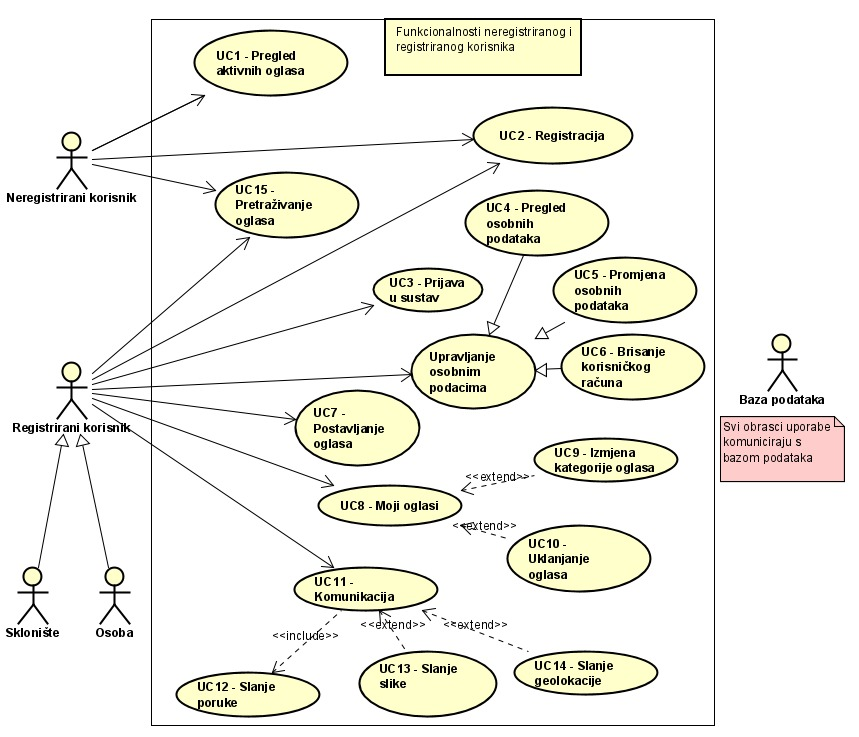
\includegraphics[width=\textwidth]{Dijagram_obrasca_uporabe.JPEG} %veličina u odnosu na širinu linije
	\caption{Dijagram obrasca uporabe, funkcionalnosti neregistriranog i registriranog korisnika}
	\label{fig:promjene6} %label mora biti drugaciji za svaku sliku
\end{figure}

\pagebreak

\subsection{Sekvencijski dijagrami}

%\textbf{\textit{dio 1. revizije}}\\

%\textit{Nacrtati sekvencijske dijagrame koji modeliraju najvažnije dijelove sustava (max. 4 dijagrama). Ukoliko postoji nedoumica oko odabira, razjasniti s asistentom. Uz svaki dijagram napisati detaljni opis dijagrama.}
%\eject

\noindent {\textbf{Obrazac uporabe UC3 - Prijava u sustav}}


\noindent{Korisnik odabire opciju "Prijavi se". Sustav prikazuje formu za prijavu, te korisnik unosi potrebne podatke. Sustav provjerava postoje li uneseni podaci u bazi podataka. Ako su uneseni podaci ispravni, sustav obavještava korisnika da je prijava uspjela te mu omogućava pristup korisničkim funkcijama. U slučaju unosa pogrešnih podataka sustav obavještava korisnika o pogrešci, te se ponovno prikazuje forma za prijavu.}
	
	
\begin{figure}[H]
	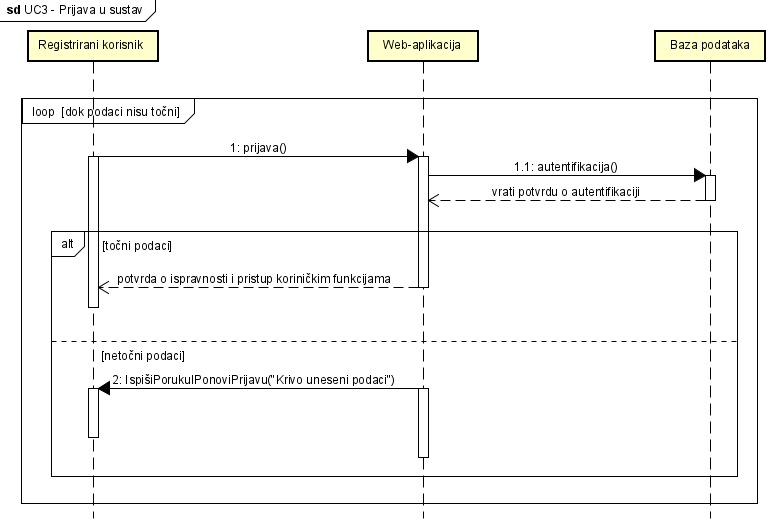
\includegraphics[width=\textwidth]{sekvencijski_dijagram_prijava_u_sustav.JPEG} %veličina u odnosu na širinu linije
	\caption{Sekvencijski dijagram za UC3}
	\label{fig:promjene3} %label mora biti drugaciji za svaku sliku
\end{figure}

\pagebreak

\noindent {\textbf{Obrazac uporabe UC7 - Postavljanje oglasa}}

\noindent{Korisnik odabire opciju "Novi oglas". Sustav prikazuje formu za unos podataka o izgubljenom kućnom ljubimcu. Korisnik unosi podatke, te odabire opciju "Spremi". Sustav provjerava u bazi podataka jesu li uneseni svi potrebni podaci. Baza podataka vraća provjeru sustavu, te ako su uneseni svi potrebni podaci za postavljanje oglasa, oglas se pohranjuje u bazu podataka i sustav obavještava korisnika da je oglas uspješno spremljen. U suprotnom, sustav obavještava korisnika da nisu uneseni svi potrebni podaci.}

\begin{figure}[H]
	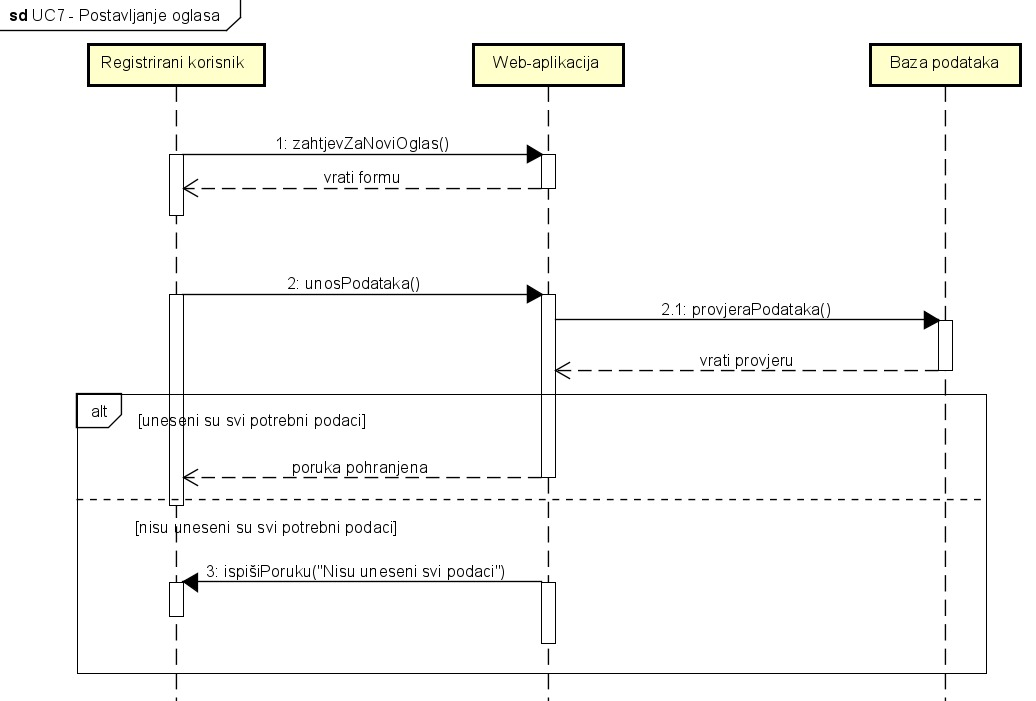
\includegraphics[width=\textwidth]{sekvencijski_dijagram_postavljanje_oglasa.JPEG} %veličina u odnosu na širinu linije
	\caption{Sekvencijski dijagram za UC7}
	\label{fig:promjen43} %label mora biti drugaciji za svaku sliku
\end{figure}

\pagebreak

\noindent {\textbf{Obrazac uporabe UC12 - Slanje poruke}}

\noindent{Kako bi korisnik poslao poruku, najprije mora odabrati oglas na kojem želi ostaviti poruku. Nakon odabira oglasa iz baze podataka se dohvaćaju podaci vezani za taj oglas. Sustav prikazuje oglas (podatke o nestalom kućnom ljubimcu). Korisnik odabire opciju "Prikaži poruke", te se iz baze podataka dohvaćaju sve dosadašnje poruke vezane za nestalog kućnog ljubimca. Sustav sada, uz podatke o ljubimcu, prikazuje i svu dosadašnju komunikaciju vezanu za nestalog kućnog ljubimca. Korisnik odabire opciju "Nova poruka" i unosi željeni tekst, te opcionalno sliku ili geolokaciju. Nakon što korisnik odabere opciju "Pošalji poruku", poruka se upisuje u bazu podataka. Nakon što je poruka uspješno upisana u bazu podataka, sustav obavještava korisnika da je poruka poslana.}

\begin{figure}[H]
	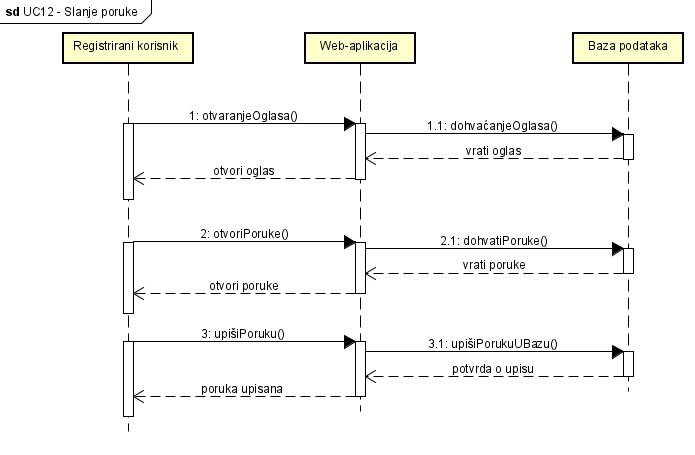
\includegraphics[width=\textwidth]{sekvencijski_dijagram_slanje_poruka.JPEG} %veličina u odnosu na širinu linije
	\caption{Sekvencijski dijagram za UC12}
	\label{fig:promjene5} %label mora biti drugaciji za svaku sliku
\end{figure}


\pagebreak

\section{Ostali zahtjevi}

%\textbf{\textit{dio 1. revizije}}\\

%\textit{Nefunkcionalni zahtjevi i zahtjevi domene primjene dopunjuju funkcionalne zahtjeve. Oni opisuju \textbf{kako se sustav treba ponašati} i koja \textbf{ograničenja} treba poštivati (performanse, korisničko iskustvo, pouzdanost, standardi kvalitete, sigurnost...). Primjeri takvih zahtjeva u Vašem projektu mogu biti: podržani jezici korisničkog sučelja, vrijeme odziva, najveći mogući podržani broj korisnika, podržane web/mobilne platforme, razina zaštite (protokoli komunikacije, kriptiranje...)... Svaki takav zahtjev potrebno je navesti u jednoj ili dvije rečenice.}

\begin{packed_item}
	\item Sustav treba omogućiti rad više korisnika u stvarnom vremenu
	\item Neispravno korištenje korisničkog sučelja ne smije narušiti funkcionalnost sustava
	\item Aplikacija treba biti izvedena kao web aplikacija prilagođena za mobilne uređaje (responzivna)
	\item Korisničko sučelje i sustav moraju podržavati hrvatsku abecedu (dijakritičke znakove) pri unosu i prikazu tekstualnog sadržaja
	\item Sustav treba biti jednostavan za korištenje
	
\end{packed_item}


	\chapter{Arhitektura i dizajn sustava}
		
		%\textbf{\textit{dio 1. revizije}}\\

		%\textit{ Potrebno je opisati stil arhitekture te identificirati: podsustave, preslikavanje na radnu platformu, spremišta podataka, mrežne protokole, globalni upravljački tok i sklopovsko-programske zahtjeve. Po točkama razraditi i popratiti odgovarajućim skicama:}
	%\begin{itemize}
		%\item 	\textit{izbor arhitekture temeljem principa oblikovanja pokazanih na predavanjima (objasniti zašto ste baš odabrali takvu arhitekturu)}
		%\item 	\textit{organizaciju sustava s najviše razine apstrakcije (npr. klijent-poslužitelj, baza podataka, datotečni sustav, grafičko sučelje)}
		%\item 	\textit{organizaciju aplikacije (npr. slojevi frontend i backend, MVC arhitektura) }		
	%\end{itemize}

	\noindent{Arhitektura se dijeli na tri podsustava:}
	\begin{packed_item}
		\item web poslužitelj
		\item web aplikaciju
		\item bazu podataka
	\end{packed_item}
	\noindent{Web aplikacije često zahtijevaju integraciju poslužitelja, aplikacije i baze podataka kako bi pružile korisnicima dinamičke i interaktivne sadržaje. \textbf{Web poslužitelj} služi kao središnja točka koja prima zahtjeve korisnika putem internetskog preglednika. \textbf{Web aplikacija} obrađuje zahtjev te ovisno o njemu komunicira s bazom podataka kako bi dohvatila, mijenjala ili pohranjivala podatke koji se koriste u procesu. \textbf{Baza podataka} je skup strukturiranih podataka koji se čuvaju na poslužitelju, a aplikacija je odgovorna za upravljanje tim podacima i osiguravanje njihove konzistentnosti. Kada se podaci mijenjaju putem aplikacije, te promjene se ažuriraju u bazi podataka, a zatim web poslužitelj šalje ažurirane informacije korisnicima putem preglednika.}
	\newline
	\noindent{Jezici korišteni pri izradi aplikacije su C\#, CSS, HTML i JavaScript.}
	\newline
	\noindent{Arhitektura sustava se bazira na \textbf{MVC} konceptu. MVC (Model-View-Controller) je arhitekturni obrazac za razvoj softverskih aplikacija. \textbf{Model} predstavlja podatke i logiku aplikacije, \textbf{View} predstavlja sučelje preko kojeg korisnici komuniciraju s aplikacijom i prikazuje im podatke iz Modela, dok \textbf{Controller} upravlja komunikacijom između Modela i View-a. Ovaj koncept omogućava jasnu organizaciju koda, razdvajanje odgovornosti između komponenti aplikacije (Model, View, Controller) te olakšava timsku suradnju i održavanje aplikacije. Zbog jasne podjele na modele, poglede i kontrolere, aplikacije izgrađene na MVC arhitekturi često su fleksibilnije i lakše za održavanje.}

	\pagebreak
				
		\section{Baza podataka}
			
			%\textbf{\textit{dio 1. revizije}}\\
			
		%\textit{Potrebno je opisati koju vrstu i implementaciju baze podataka ste odabrali, glavne komponente od kojih se sastoji i slično.}
		Za pohranu podataka iz naše web aplikacije napravljena je relacijska baza podataka. Tablicama i njihovim atributima ostvarena je komunikacija između organiziranosti, preciznosti i jednostavnog dohvaćanja podataka za daljnu obradu. Baza podataka je kreirana u SQLite-u, upravo zbog toga što se podaci iz baze mogu dijeliti između više računala i jer koristi jednu datoteku za pohranu cijele baze podataka.\\
		Baza podataka se sastoji od sljedećih entiteta:
		\begin{packed_item}
			\item User
			\item Regular
			\item Shelter
			\item TypeOfUser
			\item Communication
			\item Ad
			\item PhotoAd
			\item Pet
			\item ColorPet
			\item hasColor
		\end{packed_item}
		
			\subsection{Opis tablica}
			

				%\textit{Svaku tablicu je potrebno opisati po zadanom predlošku. Lijevo se nalazi točno ime varijable u bazi podataka, u sredini se nalazi tip podataka, a desno se nalazi opis varijable. Svjetlozelenom bojom označite primarni ključ. Svjetlo plavom označite strani ključ}
				\textbf{Korisnik (User)}
				Ovaj entitet sadržava sve primarne informacije o korisniku. Sadrži atribute: userID, userName, email, phoneNum i psw. Ovaj entitet u vezi je \textit{One-to-Many} s entitetom Ad (oglas), \textit{One-to-Many} s entitetom Communication (Komunikacija) oba preko atributa userID korisnika te u vezi \textit{One-to-One} s entitetom Regular (redovni korisnik), \textit{One-to-One} s Shelter(sklonište) i \textit{One-to-One} s TypeOfUser (tip korisnika) preko userID - korisničkog imena.
				
				
				\begin{longtblr}[
					label=none,
					entry=none
					]{
						width = \textwidth,
						colspec={|X[6,l]|X[6, l]|X[20, l]|}, 
						rowhead = 1,
					} %definicija širine tablice, širine stupaca, poravnanje i broja redaka naslova tablice
					\hline \SetCell[c=3]{c}{\textbf{User}}	 \\ \hline[3pt]
					\SetCell{LightGreen} userID & INTEGER	& jedinstveni identifikator korisnika	\\ \hline
					userName & VARCHAR & naziv korisnika u aplikaciji \\ \hline 
					email & VARCHAR & e-mail adresa korisnika\\ \hline 
					phoneNum & VARCHAR	&  broj telefona korisnika\\ \hline
					psw & VARCHAR & lozinka korisnika\\ \hline
					%\SetCell{LightBlue} primjer	& VARCHAR &   	\\ \hline 
				\end{longtblr}
				
				\textbf{Redovni korisnik (Regular)}
				Ovaj entitet sadržava informacije o regularnom korisniku. Sadrži atribute: userID, firstName - ime i lastName - prezime korisnika. Ovaj entitet u vezi je \textit{One-to-One} s entitetom User (Korisnik) preko userID korisnika.
				
				
				\begin{longtblr}[
					label=none,
					entry=none
					]{
						width = \textwidth,
						colspec={|X[6,l]|X[6, l]|X[20, l]|}, 
						rowhead = 1,
					} %definicija širine tablice, širine stupaca, poravnanje i broja redaka naslova tablice
					\hline \SetCell[c=3]{c}{\textbf{Regular}}	 \\ \hline[3pt]
					\SetCell{LightBlue} userID & INTEGER	& jedinstveni identifikator korisnika, (user.userID)	\\ \hline
					firstName & VARCHAR & ime korisnika \\ \hline 
					lastName & VARCHAR & prezime korisnika\\ \hline 
					%\SetCell{LightBlue} primjer	& VARCHAR &   	\\ \hline 
				\end{longtblr}
				
				\textbf{Sklonište (Shelter)}
				Ovaj entitet sadržava informacije o skloništu kao korisniku. Sadrži atribute: userID i nameShelter - naziv skloništa. Ovaj entitet u vezi je \textit{One-to-One} s entitetom User (Korisnik) preko userID korisnika.
				
				
				\begin{longtblr}[
					label=none,
					entry=none
					]{
						width = \textwidth,
						colspec={|X[6,l]|X[6, l]|X[20, l]|}, 
						rowhead = 1,
					} %definicija širine tablice, širine stupaca, poravnanje i broja redaka naslova tablice
					\hline \SetCell[c=3]{c}{\textbf{Shelter}}	 \\ \hline[3pt]
					\SetCell{LightBlue} userID & INTEGER	& jedinstveni identifikator korisnika, (user.userID)	\\ \hline
					nameShelter & VARCHAR & naziv skloništa za životinje \\ \hline 
					
				\end{longtblr}
				
				\textbf{Tip korisnika (TypeOfUser)}
				Ovaj entitet sadržava informacije o tipu korisnika. Korisnik može biti regular - uobičajen korisnik ili shelter - sklonište za životinje. Sadrži atribute: userID i userType - tip korisnika. Ovaj entitet u vezi je \textit{One-to-One} s entitetom User (Korisnik) preko userID korisnika.
				
				
				\begin{longtblr}[
					label=none,
					entry=none
					]{
						width = \textwidth,
						colspec={|X[6,l]|X[6, l]|X[20, l]|}, 
						rowhead = 1,
					} %definicija širine tablice, širine stupaca, poravnanje i broja redaka naslova tablice
					\hline \SetCell[c=3]{c}{\textbf{TypeOfUser}}	 \\ \hline[3pt]
					\SetCell{LightBlue} userID & INTEGER	& jedinstveni identifikator korisnika, (user.userID)	\\ \hline
					userType & VARCHAR & tip korisnika - može biti shelter ili regular \\ \hline 
					 
				\end{longtblr}
				
				\textbf{Komunikacija (Communication)}
				Ovaj entitet sadržava sve važne informacije o komunikaciji ispod aktivnog oglasa. Sadrži atribute: textID, textCom - poruka, locCom - lokacija poruke te photoCom - slika unutar poruke te adID i userID - strani ključevi tablice Ad i User. Ovaj entitet u vezi je \textit{Many-to-One} s entitetom Ad (oglas) preko atributa adID oglasa i \textit{Many-to-One} s User preko userID korisnika.
				
				
				\begin{longtblr}[
					label=none,
					entry=none
					]{
						width = \textwidth,
						colspec={|X[6,l]|X[6, l]|X[20, l]|}, 
						rowhead = 1,
					} %definicija širine tablice, širine stupaca, poravnanje i broja redaka naslova tablice
					\hline \SetCell[c=3]{c}{\textbf{Communication}}	 \\ \hline[3pt]
					\SetCell{LightGreen} textID & INTEGER & jedinstveni identifikator poruke	\\ \hline
					photoCom & VARCHAR & slika poruke\\ \hline 
					textCom & VARCHAR & tekst poruke\\ \hline 
					locCom & VARCHAR	&  lokacija poruke\\ \hline
					\SetCell{LightBlue} adID	& INTEGER &  jedinstveni identifikator oglasa, (ad.adID)	\\ \hline 
					\SetCell{LightBlue} userID	& INTEGER & jedinstveni identifikator korisnika, (user.userID) 	\\ \hline
				\end{longtblr}
				
				\textbf{Oglas (Ad)}
				Ovaj entitet sadržava sve važne informacije o postavljanju oglasa. Sadrži atribute: adID, catID - kategorija oglasa, userID - strani ključ tablice User. Ovaj entitet u vezi je \textit{Many-to-One} s entitetom User (korisnik) preko atributa userID korisnika, \textit{One-to-Many} s Communication (Komunikacija) preko atributa adID, \textit{One-to-Many} s PhotoAd (slike oglasa) preko adID,
				\textit{One-to-One} s entitetom Pet(Ljubimac) preko adID oglasa.
				
				
				\begin{longtblr}[
					label=none,
					entry=none
					]{
						width = \textwidth,
						colspec={|X[6,l]|X[6, l]|X[20, l]|}, 
						rowhead = 1,
					} %definicija širine tablice, širine stupaca, poravnanje i broja redaka naslova tablice
					\hline \SetCell[c=3]{c}{\textbf{Ad}}	 \\ \hline[3pt]
					\SetCell{LightGreen} adID & INTEGER	& jedinstveni identifikator oglasa	\\ \hline
					catAd & VARCHAR & kategorije oglasa \\ \hline 
					\SetCell{LightBlue} userID	& INTEGER & jedinstveni identifikator korisnika, (user.userID)    	\\ \hline 
				\end{longtblr}
				
				\textbf{Slike oglas (PhotoAd)}
				Ovaj entitet sadržava sve važne informacije o postavljanju slika ispod oglasa. Sadrži atribute: photoID, photo - fotografija izgubljenog ljubimca, userID - strani ključ tablice User. Ovaj entitet u vezi je \textit{Many-to-One} s entitetom Ad (Oglas) preko atributa adID. Uz to, dodano je i ograničenje na razini baze - trigger za postavljanje maksimalno 3 slika uz oglas.
				
				
				\begin{longtblr}[
					label=none,
					entry=none
					]{
						width = \textwidth,
						colspec={|X[6,l]|X[6, l]|X[20, l]|}, 
						rowhead = 1,
					} %definicija širine tablice, širine stupaca, poravnanje i broja redaka naslova tablice
					\hline \SetCell[c=3]{c}{\textbf{PhotoAd}}	 \\ \hline[3pt]
					\SetCell{LightGreen} photoID & INTEGER	& jedinstveni identifikator slike oglasa	\\ \hline
					photo & VARCHAR & fotografija ljubimca \\ \hline 
					\SetCell{LightBlue} adID	& INTEGER &  jedinstveni identifikator oglasa, (ad.adID) 	\\ \hline 
				\end{longtblr}
				
				\textbf{Ljubimac (Pet)}
				Ovaj entitet sadržava sve važne informacije o nestalom kućnom ljubimcu. Sadrži atribute: petID, namePet - ime ljubimca, dateHourMis - datum i sat nestanka, location - lokacija pri postavljanju oglasa, vrsta ljubimca species, starost age, tekstni opis description i strani ključ adID iz Ad. Ovaj entitet u vezi je \textit{One-to-One} s entitetom Ad (oglas) preko atributa adID, \textit{Many-to-Many} s ColorPet (Komunikacija) preko tablice Has.
				
				
				\begin{longtblr}[
					label=none,
					entry=none
					]{
						width = \textwidth,
						colspec={|X[6,l]|X[6, l]|X[20, l]|}, 
						rowhead = 1,
					} %definicija širine tablice, širine stupaca, poravnanje i broja redaka naslova tablice
					\hline \SetCell[c=3]{c}{\textbf{Pet}}	 \\ \hline[3pt]
					\SetCell{LightGreen} petID & INTEGER & jedinstveni identifikator ljubimca	\\ \hline
					namePet & VARCHAR & ime na koje se odaziva ljubimac \\ \hline 
					dateHourMis & DATETIME & datum i sat nestanka ljubimca\\ \hline 
					location & VARCHAR	&  geolokacija izgubljenog ljubimca\\ \hline
					species & VARCHAR & vrsta ljubimca\\ \hline
					age & VARCHAR & starost ljubimca\\ \hline
					description & VARCHAR & opis ljubimca\\ \hline
					\SetCell{LightBlue} adID	& INTEGER &  jedinstveni identifikator oglasa, (ad.adID) 	\\ \hline 
				\end{longtblr}
				
				\textbf{Boja ljubimca (ColorPet)}
				Ovaj entitet sadržava sve važne informacije o boji kućnog ljubimca. Sadrži atribute: colorID i boja ljubimca color. Ovaj entitet u vezi je \textit{Many-to-Many} s entitetom Pet(Ljubimac) preko tablice Has.
				
				
				\begin{longtblr}[
					label=none,
					entry=none
					]{
						width = \textwidth,
						colspec={|X[6,l]|X[6, l]|X[20, l]|}, 
						rowhead = 1,
					} %definicija širine tablice, širine stupaca, poravnanje i broja redaka naslova tablice
					\hline \SetCell[c=3]{c}{\textbf{ColorPet}}	 \\ \hline[3pt]
					\SetCell{LightGreen} colorID & INTEGER	& jedinstveni identifikator boje ljubimca	\\ \hline
					color & VARCHAR & boja ljubimca \\ \hline 
					
				\end{longtblr}
				
				\textbf{ImaBoju (Has)}
				Ovaj entitet spaja boju i kućnog ljubimca. Sadrži atribute jedinstvene šifre colorID i petID. Ovaj entitet u vezi je \textit{Many-to-Many} s entitetom Pet(Ljubimac) preko atributa petID te u vezi \textit{Many-to-Many} s entitetom ColorPet(boja ljubimca) preko atributa colorID.
				
				
				
				\begin{longtblr}[
					label=none,
					entry=none
					]{
						width = \textwidth,
						colspec={|X[6,l]|X[6, l]|X[20, l]|}, 
						rowhead = 1,
					} %definicija širine tablice, širine stupaca, poravnanje i broja redaka naslova tablice
					\hline \SetCell[c=3]{c}{\textbf{Has}}	 \\ \hline[3pt]
					\SetCell{LightBlue} petID	& INTEGER &  jedinstveni identifikator ljubimca, (pet.petID) \\ \hline
					\SetCell{LightBlue} colorID	& INTEGER &  jedinstveni identifikator boje ljubimca, (colorPet.colorID) 	\\ \hline 
					 
				\end{longtblr}
				
				
			
				
			
			\subsection{Dijagram baze podataka}
				%\textit{ U ovom potpoglavlju potrebno je umetnuti dijagram baze podataka. Primarni i strani ključevi moraju biti označeni, a tablice povezane. Bazu podataka je potrebno normalizirati. Podsjetite se kolegija "Baze podataka".}
				\begin{figure}
					\centering
					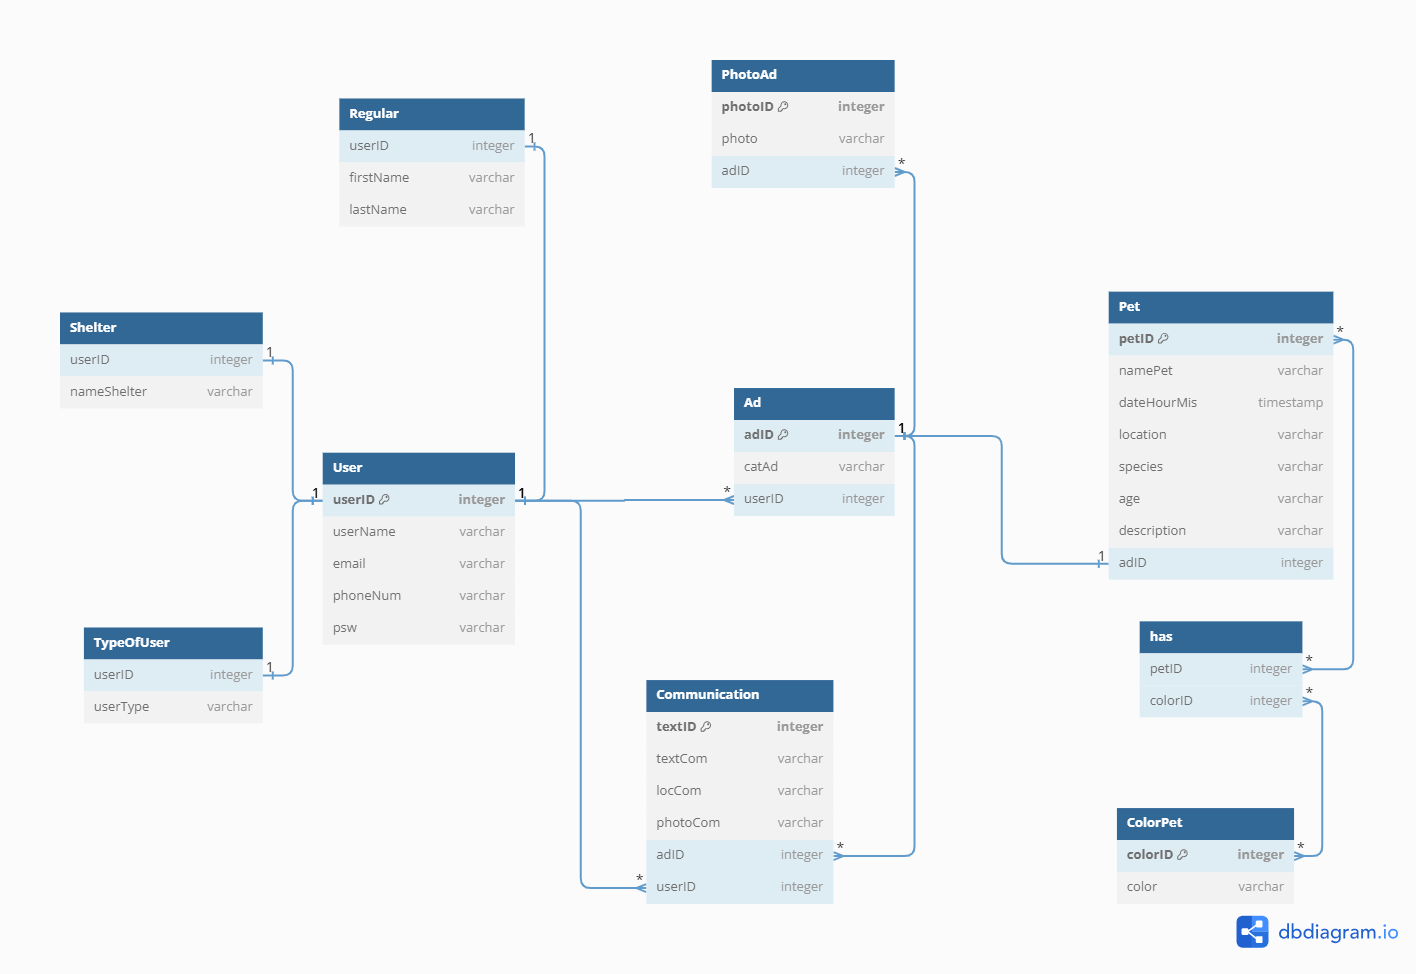
\includegraphics[width=0.8\linewidth]{ERbaza.png}
					\caption{ER dijagram baze podataka}
					\label{fig:your_label}
				\end{figure}
			
			\eject
			
			
		\section{Dijagram razreda}
		
			%\textit{Potrebno je priložiti dijagram razreda s pripadajućim opisom. Zbog preglednosti je moguće dijagram razlomiti na više njih, ali moraju biti grupirani prema sličnim razinama apstrakcije i srodnim funkcionalnostima.}\\
			
			%\textbf{\textit{dio 1. revizije}}\\
			
			%\textit{Prilikom prve predaje projekta, potrebno je priložiti potpuno razrađen dijagram razreda vezan uz \textbf{generičku funkcionalnost} sustava. Ostale funkcionalnosti trebaju biti idejno razrađene u dijagramu sa sljedećim komponentama: nazivi razreda, nazivi metoda i vrste pristupa metodama (npr. javni, zaštićeni), nazivi atributa razreda, veze i odnosi između razreda.}\\
			
			%\textbf{\textit{dio 2. revizije}}\\			
			
			%\textit{Prilikom druge predaje projekta dijagram razreda i opisi moraju odgovarati stvarnom stanju implementacije}
			
			Razredi modela odražavaju strukturu podataka unutar aplikacije, a metode koje su implementirane unutar njih služe za izravnu komunikaciju s bazom podataka kako bi dobili ili manipulirali traženim podacima. Razred Klijent predstavlja registriranog korisnika sustava s mogućnošću pristupa osnovnim funkcionalnostima sustava. Razred Sklonište ima sve funkcionalnosti kao Klijent, uz dodatnu mogućnost dodavanja kategorija oglasa. Razredi Ljubimac i Oglas sadrže informacije potrebne za stvaranje oglasa koji će biti prikazani svim korisnicima.
			
			\begin{figure}[H]
				
				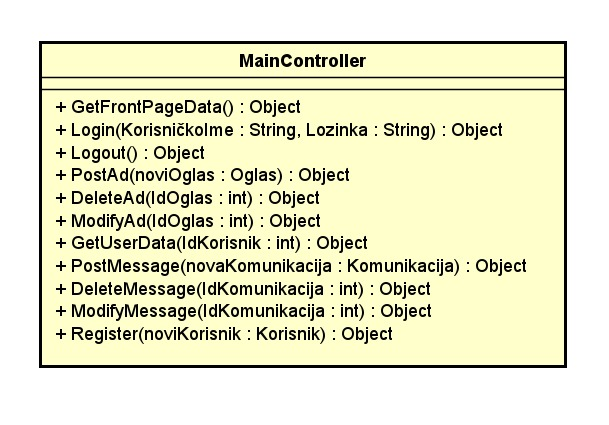
\includegraphics[scale =0.4]{kontroler.JPEG}
				\centering
				\caption{Dijagram razreda - dio Controllers}
				\label{fig:your_label}
			\end{figure}
			
			\begin{figure}[H]
				
				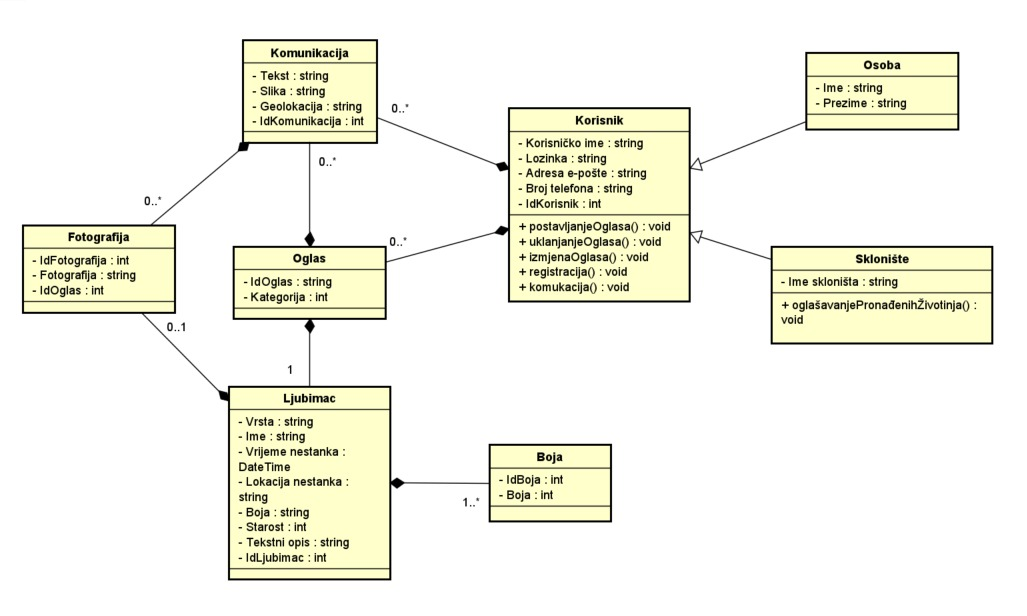
\includegraphics[scale =0.4]{model.JPEG}
				\centering
				\caption{Dijagram razreda - dio Models}
				\label{fig:your_label}
			\end{figure}
			%\eject
		
		\section{Dijagram stanja}
			
			
			\textbf{\textit{dio 2. revizije}}\\
			
			\textit{Potrebno je priložiti dijagram stanja i opisati ga. Dovoljan je jedan dijagram stanja koji prikazuje \textbf{značajan dio funkcionalnosti} sustava. Na primjer, stanja korisničkog sučelja i tijek korištenja neke ključne funkcionalnosti jesu značajan dio sustava, a registracija i prijava nisu. }
			
			
			\eject 
		
		\section{Dijagram aktivnosti}
			
			\textbf{\textit{dio 2. revizije}}\\
			
			 \textit{Potrebno je priložiti dijagram aktivnosti s pripadajućim opisom. Dijagram aktivnosti treba prikazivati značajan dio sustava.}
			
			\eject
		\section{Dijagram komponenti}
		
			\textbf{\textit{dio 2. revizije}}\\
		
			 \textit{Potrebno je priložiti dijagram komponenti s pripadajućim opisom. Dijagram komponenti treba prikazivati strukturu cijele aplikacije.}
	\chapter{Implementacija i korisničko sučelje}
		
		
		\section{Korištene tehnologije i alati}
		
			\textbf{\textit{dio 2. revizije}}
			
			 \textit{Detaljno navesti sve tehnologije i alate koji su primijenjeni pri izradi dokumentacije i aplikacije. Ukratko ih opisati, te navesti njihovo značenje i mjesto primjene. Za svaki navedeni alat i tehnologiju je potrebno \textbf{navesti internet poveznicu} gdje se mogu preuzeti ili više saznati o njima}.
			
			
			\eject 
		
	
		\section{Ispitivanje programskog rješenja}
			
			\textbf{\textit{dio 2. revizije}}\\
			
			 \textit{U ovom poglavlju je potrebno opisati provedbu ispitivanja implementiranih funkcionalnosti na razini komponenti i na razini cijelog sustava s prikazom odabranih ispitnih slučajeva. Studenti trebaju ispitati temeljnu funkcionalnost i rubne uvjete.}
	
			
			\subsection{Ispitivanje komponenti}
			\textit{Potrebno je provesti ispitivanje jedinica (engl. unit testing) nad razredima koji implementiraju temeljne funkcionalnosti. Razraditi \textbf{minimalno 6 ispitnih slučajeva} u kojima će se ispitati redovni slučajevi, rubni uvjeti te izazivanje pogreške (engl. exception throwing). Poželjno je stvoriti i ispitni slučaj koji koristi funkcionalnosti koje nisu implementirane. Potrebno je priložiti izvorni kôd svih ispitnih slučajeva te prikaz rezultata izvođenja ispita u razvojnom okruženju (prolaz/pad ispita). }
			
			
			
			\subsection{Ispitivanje sustava}
			
			 \textit{Potrebno je provesti i opisati ispitivanje sustava koristeći radni okvir Selenium\footnote{\url{https://www.seleniumhq.org/}}. Razraditi \textbf{minimalno 4 ispitna slučaja} u kojima će se ispitati redovni slučajevi, rubni uvjeti te poziv funkcionalnosti koja nije implementirana/izaziva pogrešku kako bi se vidjelo na koji način sustav reagira kada nešto nije u potpunosti ostvareno. Ispitni slučaj se treba sastojati od ulaza (npr. korisničko ime i lozinka), očekivanog izlaza ili rezultata, koraka ispitivanja i dobivenog izlaza ili rezultata.\\ }
			 
			 \textit{Izradu ispitnih slučajeva pomoću radnog okvira Selenium moguće je provesti pomoću jednog od sljedeća dva alata:}
			 \begin{itemize}
			 	\item \textit{dodatak za preglednik \textbf{Selenium IDE} - snimanje korisnikovih akcija radi automatskog ponavljanja ispita	}
			 	\item \textit{\textbf{Selenium WebDriver} - podrška za pisanje ispita u jezicima Java, C\#, PHP koristeći posebno programsko sučelje.}
			 \end{itemize}
		 	\textit{Detalji o korištenju alata Selenium bit će prikazani na posebnom predavanju tijekom semestra.}
			
			\eject 
		
		
		\section{Dijagram razmještaja}
			
			\textbf{\textit{dio 2. revizije}}
			
			 \textit{Potrebno je umetnuti \textbf{specifikacijski} dijagram razmještaja i opisati ga. Moguće je umjesto specifikacijskog dijagrama razmještaja umetnuti dijagram razmještaja instanci, pod uvjetom da taj dijagram bolje opisuje neki važniji dio sustava.}
			
			\eject 
		
		\section{Upute za puštanje u pogon}
		
			\textbf{\textit{dio 2. revizije}}\\
		
			 \textit{U ovom poglavlju potrebno je dati upute za puštanje u pogon (engl. deployment) ostvarene aplikacije. Na primjer, za web aplikacije, opisati postupak kojim se od izvornog kôda dolazi do potpuno postavljene baze podataka i poslužitelja koji odgovara na upite korisnika. Za mobilnu aplikaciju, postupak kojim se aplikacija izgradi, te postavi na neku od trgovina. Za stolnu (engl. desktop) aplikaciju, postupak kojim se aplikacija instalira na računalo. Ukoliko mobilne i stolne aplikacije komuniciraju s poslužiteljem i/ili bazom podataka, opisati i postupak njihovog postavljanja. Pri izradi uputa preporučuje se \textbf{naglasiti korake instalacije uporabom natuknica} te koristiti što je više moguće \textbf{slike ekrana} (engl. screenshots) kako bi upute bile jasne i jednostavne za slijediti.}
			
			
			 \textit{Dovršenu aplikaciju potrebno je pokrenuti na javno dostupnom poslužitelju. Studentima se preporuča korištenje neke od sljedećih besplatnih usluga: \href{https://aws.amazon.com/}{Amazon AWS}, \href{https://azure.microsoft.com/en-us/}{Microsoft Azure} ili \href{https://www.heroku.com/}{Heroku}. Mobilne aplikacije trebaju biti objavljene na F-Droid, Google Play ili Amazon App trgovini.}
			
			
			\eject 
	\chapter{Zaključak i budući rad}
		
		\textbf{\textit{dio 2. revizije}}\\
		
		 \textit{U ovom poglavlju potrebno je napisati osvrt na vrijeme izrade projektnog zadatka, koji su tehnički izazovi prepoznati, jesu li riješeni ili kako bi mogli biti riješeni, koja su znanja stečena pri izradi projekta, koja bi znanja bila posebno potrebna za brže i kvalitetnije ostvarenje projekta i koje bi bile perspektive za nastavak rada u projektnoj grupi.}
		
		 \textit{Potrebno je točno popisati funkcionalnosti koje nisu implementirane u ostvarenoj aplikaciji.}
		
		\eject 
	\chapter*{Popis literature}
		\addcontentsline{toc}{chapter}{Popis literature}
	 	
 		\textbf{\textit{Kontinuirano osvježavanje}}
	
		\textit{Popisati sve reference i literaturu koja je pomogla pri ostvarivanju projekta.}
		
		
		\begin{enumerate}
			
			
			\item  Programsko inženjerstvo, FER ZEMRIS, \url{http://www.fer.hr/predmet/proinz}
			
			\item  I. Sommerville, "Software engineering", 8th ed, Addison Wesley, 2007.
			
			\item  T.C.Lethbridge, R.Langaniere, "Object-Oriented Software Engineering", 2nd ed. McGraw-Hill, 2005.
			
			\item  I. Marsic, Software engineering book``, Department of Electrical and Computer Engineering, Rutgers University, \url{http://www.ece.rutgers.edu/~marsic/books/SE}
			
			\item  The Unified Modeling Language, \url{https://www.uml-diagrams.org/}
			
			\item  Astah Community, \url{http://astah.net/editions/uml-new}
		\end{enumerate}
		
		 
	
	
	\begingroup
	\renewcommand*\listfigurename{Indeks slika i dijagrama}
	%\renewcommand*\listtablename{Indeks tablica}
	%\let\clearpage\relax
	\listoffigures
	%\vspace{10mm}
	%\listoftables
	\endgroup
	\addcontentsline{toc}{chapter}{Indeks slika i dijagrama}


	
	\eject 
		
	\chapter*{Dodatak: Prikaz aktivnosti grupe}
		\addcontentsline{toc}{chapter}{Dodatak: Prikaz aktivnosti grupe}
		
		\section*{Dnevnik sastajanja}
		
		\textbf{\textit{Kontinuirano osvježavanje}}\\
		
		 %\textit{U ovom dijelu potrebno je redovito osvježavati dnevnik sastajanja prema predlošku.}
		
		\begin{packed_enum}
			\item  sastanak
			
			\item[] \begin{packed_item}
				\item Datum: 18. listopada 2023.
				\item Prisustvovali: Mia Krstičević, Filip Smolić, Toni Vanjak, Fran Kufrin, Dominik Šarić, Vito Tomas, Lucija Renić
				\item Teme sastanka:
				\begin{packed_item}
					\item  općenito o zadatku
					\item  alati i tehnologije
				\end{packed_item}
			\end{packed_item}
			
			\item  sastanak
			\item[] \begin{packed_item}
				\item Datum: 23. listopada 2023.
				\item Prisustvovali: Mia Krstičević, Filip Smolić, Toni Vanjak, Fran Kufrin, Dominik Šarić, Vito Tomas, Lucija Renić
				\item Teme sastanka:
				\begin{packed_item}
					\item  funkcionalnosti
					\item  zahtjevi
					\item  alati i tehnologije
				\end{packed_item}
			\end{packed_item}
			
			\item  sastanak
			\item[] \begin{packed_item}
				\item Datum: 2. studenoga 2023.
				\item Prisustvovali: Mia Krstičević, Filip Smolić, Toni Vanjak, Fran Kufrin, Dominik Šarić, Vito Tomas, Lucija Renić
				\item Teme sastanka:
				\begin{packed_item}
					\item  alati i tehnologije
					\item baza podataka
				\end{packed_item}
			\end{packed_item}
			
			\item  sastanak
			\item[] \begin{packed_item}
				\item Datum: 9. studenoga 2023.
				\item Prisustvovali: Mia Krstičević, Filip Smolić, Toni Vanjak, Fran Kufrin, Dominik Šarić, Vito Tomas, Lucija Renić
				\item Teme sastanka:
				\begin{packed_item}
					\item dosadašnji napredak
					\item arhitektura
				\end{packed_item}
			\end{packed_item}
			
			\item  sastanak
			\item[] \begin{packed_item}
				\item Datum: 14. studenoga 2023.
				\item Prisustvovali: Mia Krstičević, Filip Smolić, Toni Vanjak, Fran Kufrin, Dominik Šarić, Vito Tomas, Lucija Renić
				\item Teme sastanka:
				\begin{packed_item}
					\item dosadašnji napredak
					\item dijagram razreda
				\end{packed_item}
			\end{packed_item}
			
			%
			
		\end{packed_enum}
		
		\eject
		\section*{Tablica aktivnosti}
		
			\textbf{\textit{Kontinuirano osvježavanje}}\\
			
			 \textit{Napomena: Doprinose u aktivnostima treba navesti u satima po članovima grupe po aktivnosti.}

			\begin{longtblr}[
					label=none,
				]{
					vlines,hlines,
					width = \textwidth,
					colspec={X[7, l]X[1, c]X[1, c]X[1, c]X[1, c]X[1, c]X[1, c]X[1, c]}, 
					vline{1} = {1}{text=\clap{}},
					hline{1} = {1}{text=\clap{}},
					rowhead = 1,
				} 
			
				\SetCell[c=1]{c}{} & \SetCell[c=1]{c}{\rotatebox{90}{\textbf{Mia Krstičević}}} & \SetCell[c=1]{c}{\rotatebox{90}{\textbf{Filip Smolić }}} &	\SetCell[c=1]{c}{\rotatebox{90}{\textbf{Toni Vanjak }}} & \SetCell[c=1]{c}{\rotatebox{90}{\textbf{Fran Kufrin }}} &	\SetCell[c=1]{c}{\rotatebox{90}{\textbf{Dominik Šarić }}} & \SetCell[c=1]{c}{\rotatebox{90}{\textbf{Vito Tomas }}} &	\SetCell[c=1]{c}{\rotatebox{90}{\textbf{Lucija Renić }}} \\  
				Upravljanje projektom 		&30  &  &  &  &  &  & \\ 
				Opis projektnog zadatka 	&  &  &  &  &  &  &7 \\ 
				
				Funkcionalni zahtjevi       &  &  &  &  &  &  &3  \\ 
				Opis pojedinih obrazaca 	&  &  &  &  &  &  &11  \\ 
				Dijagram obrazaca 			&  &  &5  &  &  &  &1  \\ 
				Sekvencijski dijagrami 		&  &  &7  &  &  &  &1  \\ 
				Opis ostalih zahtjeva 		&  &  &  &  &  &  &2  \\ 
				Arhitektura i dizajn sustava	 &  &6  &  &  &  &  &4  \\ 
				Baza podataka				&10  &  &  &  &  &  &   \\ 
				Dijagram razreda 			&  &  &5  &  &  &  &   \\ 
				Dijagram stanja				&  &  &  &  &  &  &  \\ 
				Dijagram aktivnosti 		&  &  &  &  &  &  &  \\ 
				Dijagram komponenti			&  &  &  &  &  &  &  \\ 
				Korištene tehnologije i alati 		&  &  &  &  &  &  &  \\ 
				Ispitivanje programskog rješenja 	&  &  &  &  &  &  &  \\ 
				Dijagram razmještaja			&  &  &  &  &  &  &  \\ 
				Upute za puštanje u pogon 		&  &  &  &  &  &  &  \\  
				Dnevnik sastajanja 			&  &  &  &  &  &  &2  \\ 
				Zaključak i budući rad 		&  &  &  &  &  &  &  \\  
				Popis literature 			&  &  &  &  &  &  &  \\  
				&  &  &  &  &  &  &  \\ \hline 
				\textit{Dodatne stavke kako ste podijelili izradu aplikacije} 			&  &  &  &  &  &  &  \\ 
				\textit{front end} 				&  &80  &  &80  &  &  &  \\  
				\textit{izrada baze podataka} 		 			&60  &  &  &  &  &  & \\  
				\textit{spajanje s bazom podataka} 							&  &  &  &  &27  &30  &  \\ 
				\textit{back end} 							&  &  &  &  &58  &60  &  \\  
				 							&  &  &  &  &  &  &\\ 
			\end{longtblr}
					
					
		\eject
		\section*{Dijagrami pregleda promjena}
		
		\textbf{\textit{dio 2. revizije}}\\
		
		\textit{Prenijeti dijagram pregleda promjena nad datotekama projekta. Potrebno je na kraju projekta generirane grafove s gitlaba prenijeti u ovo poglavlje dokumentacije. Dijagrami za vlastiti projekt se mogu preuzeti s gitlab.com stranice, u izborniku Repository, pritiskom na stavku Contributors.}
		
	


\end{document} %naredbe i tekst nakon ove naredbe ne ulaze u izgrađen dokument 


